\section{Intro exercise}
\begin{figure}[!ht]
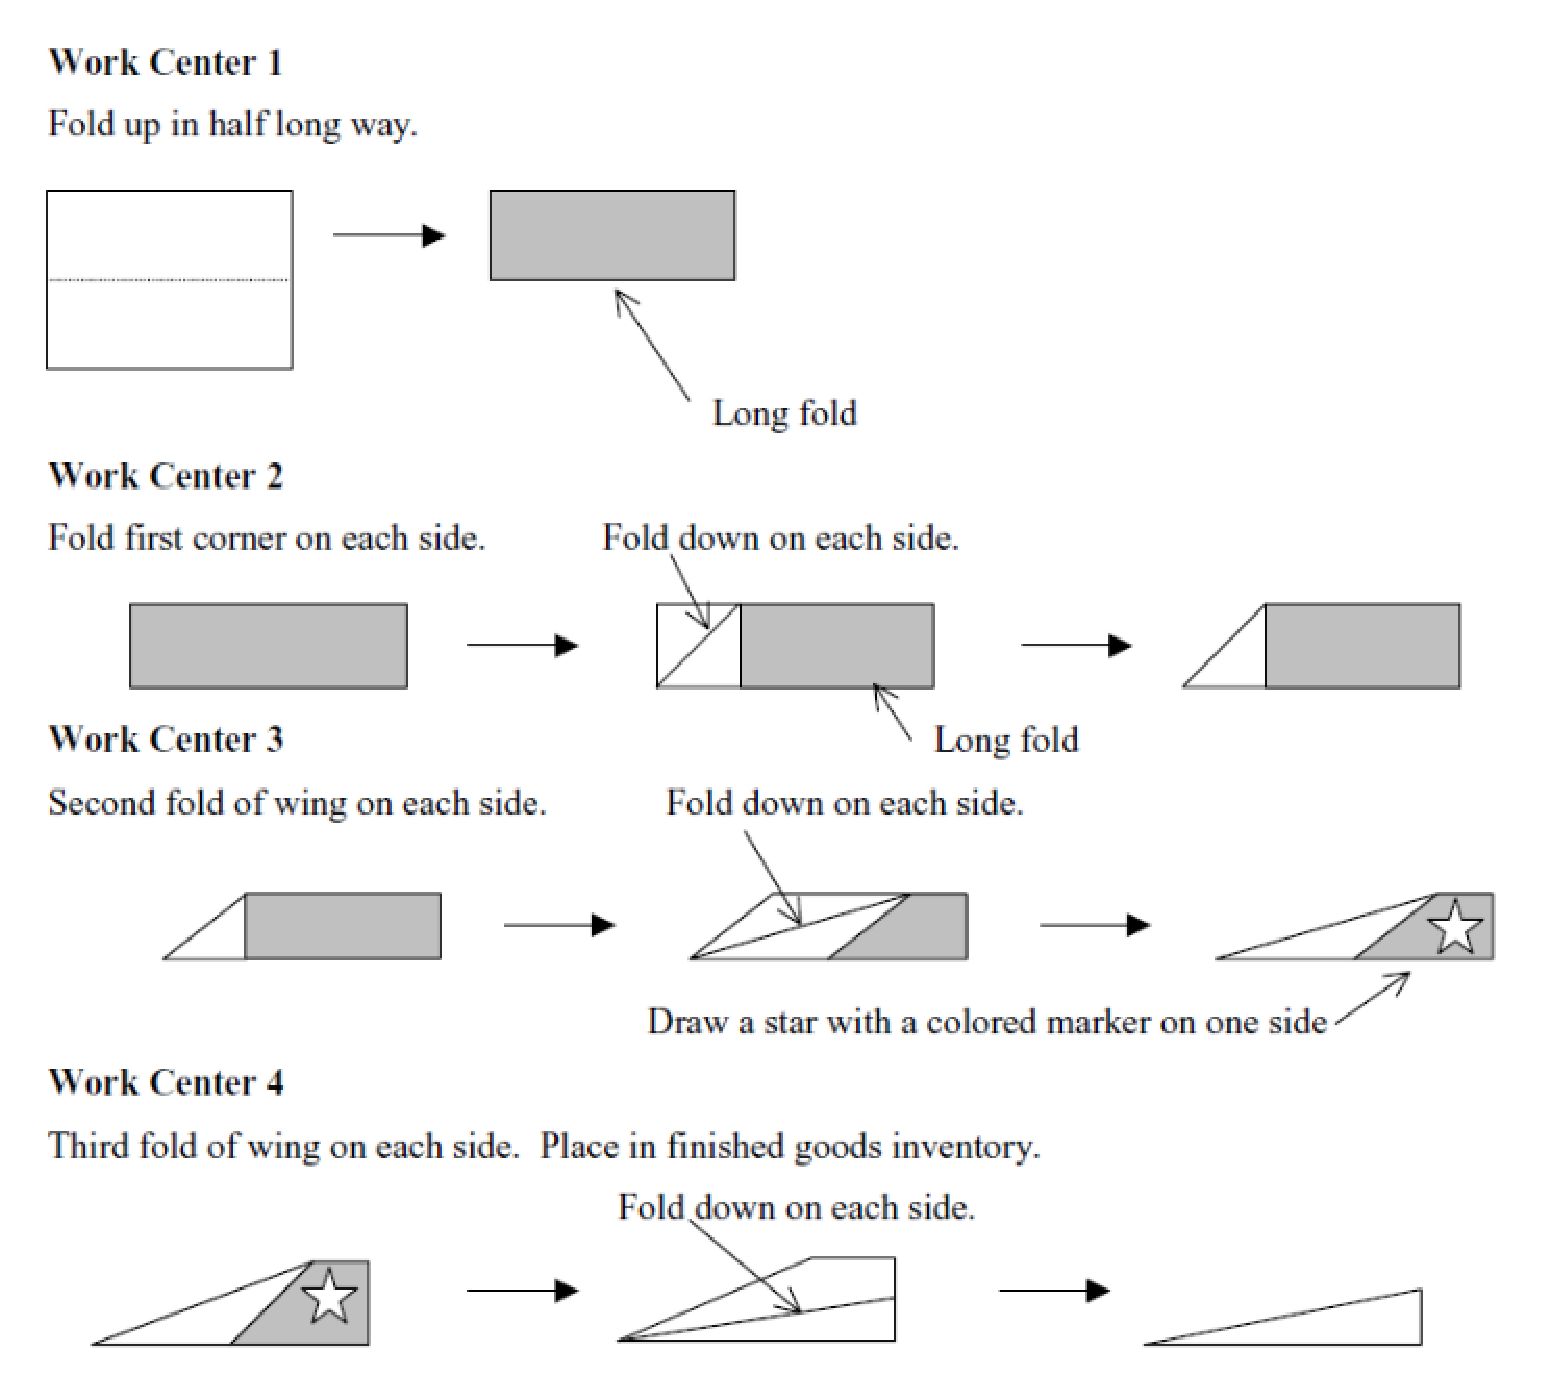
\includegraphics[width=\textwidth]{intro-exercise.eps}
\end{figure}

\subsection{Assignment}

\begin{flushleft}
\textbf{a. Which work center has a bottleneck? Why?}

The main bottleneck is between Work Center 3 and 4.
That is because in Work Center 3, 2 steps are required, whereas in 1, 2 and 4, 1 step is required. (if we assume that the non-long folds take as long as 1 long fold)

The bottleneck means that whenever Work Center 3 deliveres a paper plane, 2 planes has been delivered from Work Center 2.
This means that a stack of planes will build up in Work Center 3, and the effectiveness is hindered.
\end{flushleft}

\begin{flushleft}
\textbf{b. What should be done to reduce bottlenecks in a production line?}

A solution to this bottleneck could be to order paper with a star already printed on, so the step would disappear altogether.

Another solution could be to move the task into Work Center 1, although that would make Work Center 1 take longer to produce a folded plane.
\end{flushleft}
